\documentclass{article}
\usepackage{graphicx} 
\usepackage{amsmath}
\usepackage{float}
\graphicspath{{images/}}

\title{\textbf{Power Electronics Laboratory 
\\Session 4: DC-AC converter 1}}
\author{Team 3 :
 \\Po Ting Yeh K-9056
\\Beyazit Bilal Ozkaya 341967
 \\Braulio Cardenas 342021}
\date{}

\begin{document}

\maketitle

\section*{Introduction}
This experiment explores the fundamental operation and characteristics of DC-AC power converters. In the first part, we analyze a half-bridge converter topology. We test the system using different modulation indexes ($m_a$) to mathematically calculate and simulate the fundamental components of the output voltage, output current, and active power. This part also uses Fast Fourier Transform (FFT) to analyze the frequency spectrum, allowing us to identify the switching frequency and observe how the RL load filters out high-frequency current harmonics.
In the second part, we implement an H-Bridge converter. The main focus of this section is to compare bipolar and unipolar Pulse Width Modulation (PWM) techniques. We evaluate how these different modulation strategies impact the harmonic distortion, voltage transitions, and the overall quality of the output waveforms. Finally, across both topologies, we measure the input and output active power to practically confirm that the systems obey the principle of energy conservation. 

\section{Part 1}
\begin{figure}[H]
    \centering
    
\includegraphics[width=1\linewidth]{img1.png}
    \caption{ Half-Bridge Converter topology and modulation scheme}
    \label{fig:placeholder}
\end{figure}
\subsection*{Tasks:}
\subsection{Task 1}

\begin{table}[h!]
\centering
\begin{tabular}{|c|c|}
\hline
\textbf{s1 (On-OFF)} & \textbf{vconv} \\ \hline
1 (on)  & $+\frac{V_{dc}}{2}$ (+250V) \\ \hline
0 (off) & $-\frac{V_{dc}}{2}$ (-250V) \\ \hline
\end{tabular}
\caption{Relation between s1 states and $V_{conv}$ }
\end{table}

\subsection{Task 2: (Figure 1)}
\subsection{Task 3:}
To analyze the performance of the half-bridge converter, three different modulation indexes ($m_a$) were selected: 1.0, 0.8, and 0.4.
\subsubsection{Load Impedance Calculation}
Before evaluating the specific cases, the load impedance ($Z$) at the fundamental frequency ($f = 50\text{Hz}$) must be determined.
Given $R = 10\Omega$ and $L = 10\text{mH}$:
\begin{itemize}
    \item $Z = R + j\omega L = 10 + j(2\pi \cdot 50 \cdot 0.01) = 10 + j3.1416\Omega$
\end{itemize}
\begin{itemize}
    \item Impedance Magnitude: $|Z| = \sqrt{10^2 + 3.1416^2} \approx \mathbf{10.48\Omega}$
\end{itemize}
\subsubsection{Theoretical Justification and Simulation Verification }
The fundamental component of the output voltage peak is calculated as $V_{out, peak} = m_a \cdot \frac{V_{dc}}{2}$ (where $V_{dc}/2 = 250\text{V}$). The fundamental current peak is $I_{out, peak} = \frac{V_{out, peak}}{|Z|}$. Finally, the active power delivered to the load is purely consumed by the resistor, calculated using the RMS current: $P_{active} = I_{out, rms}^2 \cdot R = (\frac{I_{out, peak}}{\sqrt{2}})^2 \cdot 10$.
	\\\\\begin{tabular}{c}
	     Case 1: $m_a = 1.0$
	\end{tabular} 
\begin{itemize}
    \item Voltage ($V_{out, peak}$): Theoretical $= 1.0 \cdot 250 = \mathbf{250\text{V}}$. The Fourier analysis table verifies this exactly at 250V.
\end{itemize}
\begin{itemize}
    \item Current ($I_{out, peak}$): Theoretical $= 250\text{V} / 10.48\Omega = \mathbf{23.85\text{A}}$. The simulation accurately displays a peak of 23.8 A.
\end{itemize}
\begin{itemize}
    \item Active Power ($P$): Theoretical $= (\frac{23.85}{\sqrt{2}})^2 \cdot 10 \approx \mathbf{2842\text{W}}$. The power measurement block in the simulation strongly aligns with this value.
\end{itemize}
\begin{figure}[H]
    \centering
    
\includegraphics[width=0.75\linewidth]{img2.png}
    \caption{Frequency spectrum for modulation index m = 1.0}
    \label{fig:placeholder}
\end{figure}
\begin{figure}[H]
    \centering
    
\includegraphics[width=1\linewidth]{img3.png}
    \caption{m = 1.0}
    \label{fig:placeholder}
\end{figure}

\\ Case 2: $m_a = 0.8$
\begin{itemize}
    \item Voltage ($V_{out, peak}$): Theoretical $= 0.8 \cdot 250 = \mathbf{200\text{V}}$. Verified by the simulation's 50Hz Fourier component.
\end{itemize}
\begin{itemize}
    \item Current ($I_{out, peak}$): Theoretical $= 200\text{V} / 10.48\Omega = \mathbf{19.08\text{A}}$. Confirmed by the measured current waveform.
\end{itemize}
\begin{itemize}
    \item Active Power ($P$): Theoretical $= (\frac{19.08}{\sqrt{2}})^2 \cdot 10 \approx \mathbf{1820\text{W}}$. The simulation effectively matches this active power delivery.
\end{itemize}
\begin{figure}[H]
    \centering
    
\includegraphics[width=0.75\linewidth]{img4.png}
    \caption{Frequency spectrum for modulation index m = 0.8}
    \label{fig:placeholder}
\end{figure}
\begin{figure}[H]
    \centering
    
\includegraphics[width=1\linewidth]{img5.png}
    \caption{m = 0.8}
    \label{fig:placeholder}
\end{figure}
\\Case 3: $m_a = 0.4$
\begin{itemize}
    \item Voltage ($V_{out, peak}$): Theoretical $= 0.4 \cdot 250 = \mathbf{100\text{V}}$. Verified by simulation.
\end{itemize}
\begin{itemize}
    \item Current ($I_{out, peak}$): Theoretical $= 100\text{V} / 10.48\Omega = \mathbf{9.54\text{A}}$. Confirmed by simulation.
\end{itemize}
\begin{itemize}
    \item Active Power ($P$): Theoretical $= (\frac{9.54}{\sqrt{2}})^2 \cdot 10 \approx \mathbf{455\text{W}}$. The simulated periodic average power confirms this analytical result.
\end{itemize}
\begin{figure}[H]
    \centering
    
\includegraphics[width=0.75\linewidth]{img6.png}
    \caption{Frequency spectrum for modulation index m = 0.4}
    \label{fig:placeholder}
\end{figure}
\begin{figure}[H]
    \centering
    
\includegraphics[width=1\linewidth]{img7.png}
    \caption{m = 0.4}
    \label{fig:placeholder}
\end{figure}
    \textbf{Comment:} Across all three modulation indexes, the simulated fundamental components and active power values flawlessly match the mathematical calculations. This validates that the half-bridge converter successfully operates as a linear amplifier for the fundamental frequency, where the output amplitude is directly and linearly controlled by the modulation index ($m_a$).
\\
\subsection{Task 4:}
To measure the total input active power ($P_{in}$), the instantaneous power delivered by both the upper and lower 250V DC sources was calculated ($P_{in} = V_{dc,top} \cdot I_{in,top} + V_{dc,bot} \cdot I_{in,bot}$) and then averaged over a 50Hz period.
Using $m_a = 1.0$ as an example, the simulation displays the following results:
Input Active Power ($P_{in}$): Approximately 2844.76 W.
Total Output Active Power ($P_{out}$): Approximately 2844.76 W.
Fundamental Output Power ($P_1$): 2842W (calculated in Task 3).
\begin{figure}[H]
    \centering
    
\includegraphics[width=1\linewidth]{img8.png}
    \caption{Converter topology, active power calculation}
    \label{fig:placeholder}
\end{figure}

\textbf{Comment:} Comparing the results, the total input active power ($P_{in}$) is perfectly equal to the total output active power ($P_{out}$). This indicates a theoretical efficiency of exactly 100\%, which perfectly aligns with the simulation conditions since ideal IGBT and diode models (zero conduction and switching losses) were used. Furthermore, it is important to note that the total active power ($P_{in} = P_{out}$) is slightly higher than the fundamental active power ($2842\text{W}$). This extra power corresponds to the harmonic power dissipation. The high-frequency PWM switching introduces harmonic currents which flow through the $10\Omega$ load resistor, generating additional real power loss ($P_{harmonics} = \sum I_{n,rms}^2 \cdot R$). Thus, the energy conservation is fully validated: $P_{in} = P_{fundamental} + P_{harmonics}$.

\subsection{Task 5:}
To obtain the frequency spectrum, the Fourier analysis tool was applied to the steady-state voltage and current waveforms. The base frequency was set to 50 Hz, and the spectrum was plotted up to 50 kHz (1000 harmonics).
\subsubsection{Identifying the Switching Frequency}
By observing the voltage spectrum ($v_{conv}$), a dominant fundamental component is clearly visible at 50 Hz. Beyond the fundamental frequency, the spectrum remains mostly flat until a large cluster of harmonic components appears exactly at 10,000 Hz (10 kHz). Additional sidebands and clusters also appear at multiples of this frequency (e.g., 20 kHz, 30 kHz, 40 kHz). Therefore, the switching frequency ($f_s$) of the PWM is successfully identified as 10 kHz, which perfectly matches the system parameters.
\begin{figure}[H]
    \centering
    
\includegraphics[width=0.75\linewidth]{img9.png}
    \caption{Frequency spectrum}
    \label{fig:placeholder}
\end{figure}
\subsubsection{Comments on Voltage and Current Spectrums}
\begin{itemize}
    \item Voltage Spectrum ($v_{conv}$): The spectrum mathematically confirms the principle of PWM. The modulation process shifts the unwanted harmonic energy far away from the 50 Hz fundamental frequency, concentrating it around the 10 kHz switching frequency and its multiples.
\end{itemize}
\begin{itemize}
    \item Current Spectrum ($i_{out}$): Unlike the voltage spectrum, the current spectrum shows almost no harmonic content at 10 kHz. This is due to the low-pass filtering effect of the series RL load. The impedance of the $10\text{mH}$ inductor is highly frequency-dependent ($Z_L = 2\pi f L$). At the fundamental frequency (50 Hz), the inductive reactance is only $3.14\Omega$, allowing the 50 Hz current to pass easily. However, at the switching frequency (10 kHz), the reactance increases massively to approximately $628\Omega$. This high impedance effectively blocks the high-frequency voltage harmonics from generating high-frequency currents, resulting in a smooth, highly sinusoidal output current waveform.
\end{itemize}

\section{Part 2}
This section analyzes the operation of the H-Bridge DC-AC converter using different modulation techniques. The impact of bipolar and unipolar PWM strategies on the output voltage, current, and harmonic content is evaluated.
\subsection*{Tasks:}
\subsection{Task 1:}
The H-Bridge converter consists of four switches, allowing different switching states. Depending on the combination of switches, the output voltage can be +Vdc, -Vdc, or 0.
\begin{table}[h!]
\centering
\begin{tabular}{|c|c|c|}
\hline
\textbf{s1 (On-OFF)} & \textbf{s2 (On-OFF)} & \textbf{$V_{conv}$ (V)} \\ \hline
On  & Off & 500  \\ \hline
Off & On  & -500 \\ \hline
On  & On  & 0    \\ \hline
Off & Off & 0    \\ \hline
\end{tabular}
\caption{Switching states of $s_1$ and $s_2$ and converter voltage($V_{conv}$)}
\end{table}
\begin{figure}[H]
    \centering
    
\includegraphics[width=0.75\linewidth]{img10.png}
    \caption{s1: ON, s2: OFF}
    \label{fig:placeholder}
\end{figure}
\begin{figure}[H]
    \centering
    
\includegraphics[width=0.75\linewidth]{img11.png}
    \caption{s1: OFF, s2: ON}
    \label{fig:placeholder}
\end{figure}
\begin{figure}[H]
    \centering
    
\includegraphics[width=0.75\linewidth]{img12.png}
    \caption{s1: ON, s2: ONN}
    \label{fig:placeholder}
\end{figure}
\begin{figure}[H]
    \centering
    
\includegraphics[width=0.75\linewidth]{img13.png}
    \caption{s1: OFF, s2: OFF}
    \label{fig:placeholder}
\end{figure}
The H-Bridge topology allows bidirectional voltage generation, which is essential for AC output synthesis.
\\
\subsection{Task 2:}
The H-Bridge converter was implemented using bipolar PWM modulation. In this scheme, the output voltage switches directly between +Vdc and -Vdc depending on the comparison between the reference and carrier signals.
\begin{figure}[H]
    \centering
    
\includegraphics[width=1\linewidth]{img14.png}
    \caption{H-Bridge Converter Topology and Bipolar modulation scheme}
    \label{fig:placeholder}
\end{figure}
\begin{figure}[H]
    \centering
    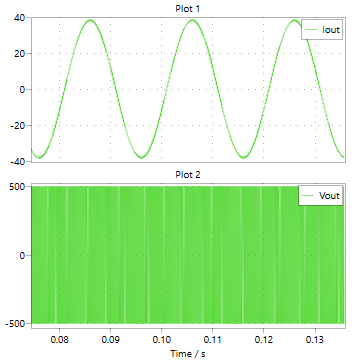
\includegraphics[width=0.75\linewidth]{img15.png}
    \caption{Plot of the output current and voltage}
    \label{fig:placeholder}
\end{figure}
Bipolar modulation is simple to implement but produces higher harmonic distortion due to large voltage transitions.
\subsection{Task 3:}
The converter was implemented using unipolar PWM modulation. In this case, each leg of the H-Bridge is modulated separately, producing three voltage levels: +Vdc, 0, and -Vdc.
\begin{figure}[H]
    \centering
    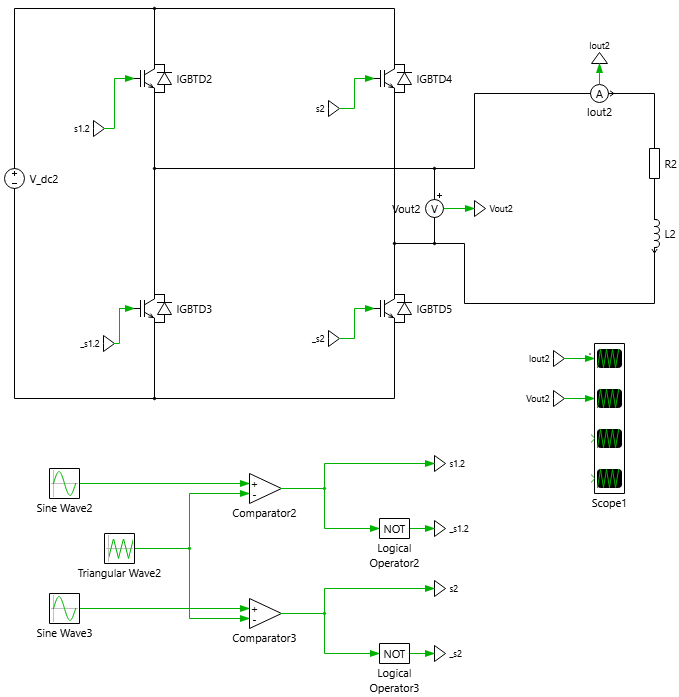
\includegraphics[width=1\linewidth]{img16.png}
    \caption{H-Bridge Converter Topology and  Unipolar modulation scheme}
    \label{fig:placeholder}
\end{figure}
Compared to bipolar modulation, the voltage transitions are smaller, reducing harmonic distortion.
\begin{figure}
    \centering
    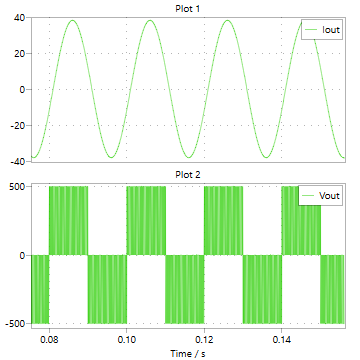
\includegraphics[width=0.75\linewidth]{img17.png}
    \caption{Plot of the output current and voltage}
    \label{fig:placeholder}
\end{figure}
Unipolar modulation improves the quality of the output waveform by reducing low-order harmonics.
\subsection{Task 4:}
Three different modulation indexes were selected to analyze the converter performance. For each case, the fundamental component of the output voltage, current, and the delivered active power were calculated and verified through simulation.
\begin{table}[h!]
\centering
\begin{tabular}{|c|c|c|c|}
\hline
\textbf{Modulation Index (m)} & \textbf{$V_{RMS}$ (V)} & \textbf{$I_{RMS}$ (A)} & \textbf{$P$ (W)} \\ \hline
0.5 & 176.77 & 16.86 & 2840  \\ \hline
0.8 & 282.84 & 26.98 & 7280  \\ \hline
1.0 & 353.55 & 33.73 & 11370 \\ \hline
\end{tabular}
\caption{Calculated RMS voltage, current, and power for 3 modulation index}
\end{table}

As the modulation index increases, the output voltage and current also increase, resulting in higher active power.

\begin{table}[h!]
\centering
\begin{tabular}{|c|c|c|c|}
\hline
\textbf{Modulation Index (m)} & \textbf{$V_{RMS}$ (V)} & \textbf{$I_{RMS}$ (A)} & \textbf{$P$ (W)} \\ \hline
0.5 & 278.55 & 16.57 & 2726  \\ \hline
0.8 & 352.3  & 26.5  & 6979  \\ \hline
1.0 & 393.9  & 33.15 & 10904 \\ \hline
\end{tabular}
\caption{Simulation values of RMS voltage, current, and power for each modulation index}
\end{table}
\begin{figure}[H]
    \centering
    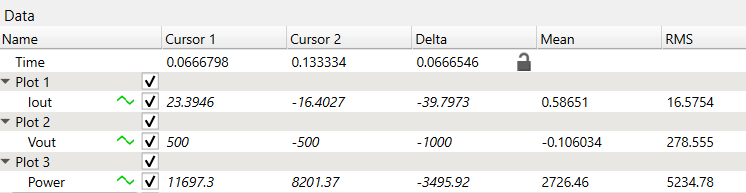
\includegraphics[width=0.75\linewidth]{img18.png}
    \caption{m = 0.5}
    \label{fig:placeholder}
\end{figure}
\begin{figure}[H]
    \centering
    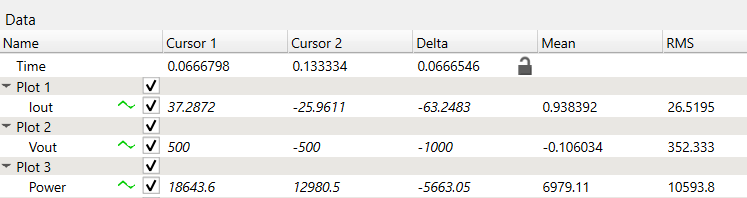
\includegraphics[width=0.75\linewidth]{img19.png}
    \caption{m = 0.8}
    \label{fig:placeholder}
\end{figure}
\begin{figure}[H]
    \centering
    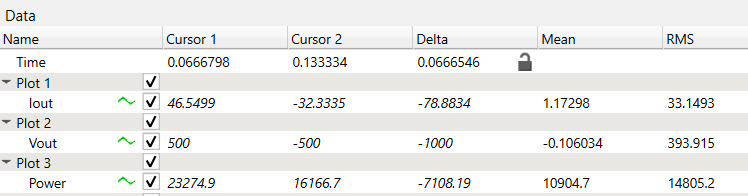
\includegraphics[width=0.75\linewidth]{img20.png}
    \caption{m = 1}
    \label{fig:placeholder}
\end{figure}
The modulation index directly controls the amplitude of the output voltage and consequently the delivered power.

\subsection{Task 5:}
The input active power was measured from the DC side using the instantaneous voltage and current. The output active power was obtained from the load side.
\begin{figure}[H]
    \centering
    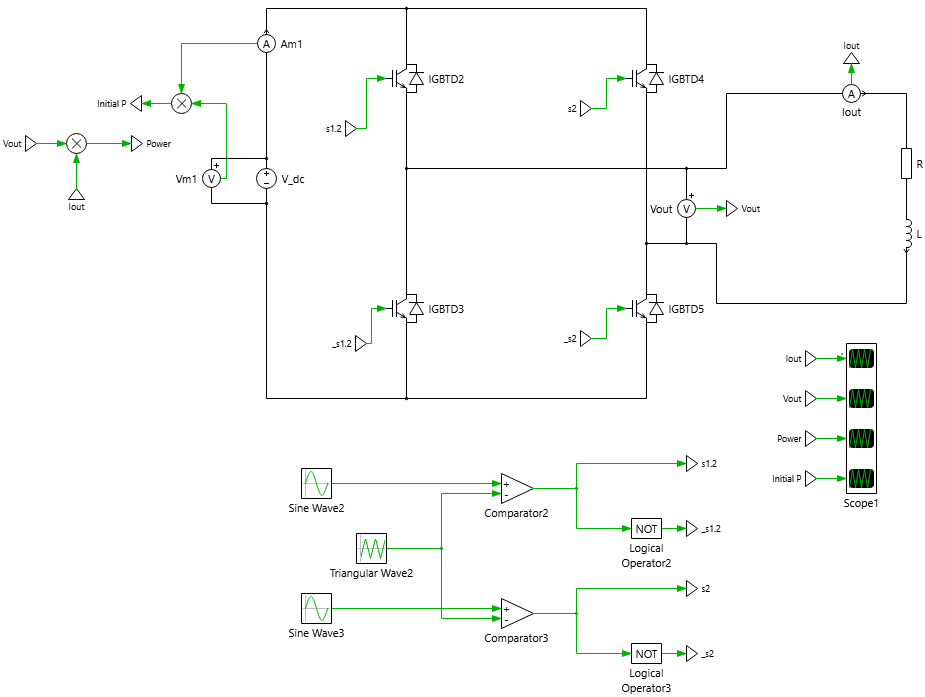
\includegraphics[width=1\linewidth]{img21.png}
    \caption{ H-Bridge Converter Topology, Power calculation}
    \label{fig:placeholder}
\end{figure}
\begin{figure}[H]
    \centering
    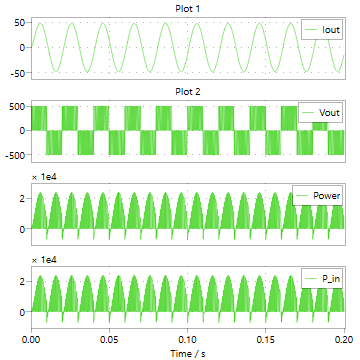
\includegraphics[width=0.75\linewidth]{img22.png}
    \caption{Plot of input Vs output active power }
    \label{fig:placeholder}
\end{figure}
\textbf{Comment:} The input and output powers were found to be approximately equal.
This confirms the energy conservation principle in the converter. Small differences may be due to numerical errors and harmonic components.
\subsection{Task 6:}
The frequency spectrum of the output voltage and current was obtained using FFT analysis for both bipolar and unipolar modulation.
\begin{figure}[H]
    \centering
    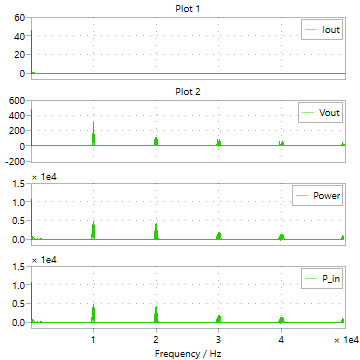
\includegraphics[width=0.75\linewidth]{img23.png}
    \caption{Bipolar Modulation Freq. Spectrum}
    \label{fig:placeholder}
\end{figure}
\begin{figure}[H]
    \centering
    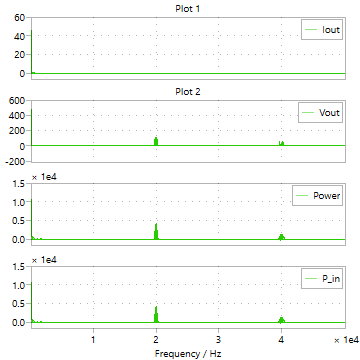
\includegraphics[width=0.75\linewidth]{img24.png}
    \caption{Unipolar Modulation Freq. Spectrum}
    \label{fig:placeholder}
\end{figure}
\begin{itemize}
    \item The fundamental frequency at 50 Hz is clearly observed in all cases.
\end{itemize}
\begin{itemize}
    \item In bipolar modulation, the dominant harmonics appear around the switching frequency (10 kHz).
\end{itemize}
\begin{itemize}
    \item In unipolar modulation, the dominant harmonics are shifted to higher frequencies (around 20 kHz).
\end{itemize}
\begin{itemize}
    \item Unipolar modulation results in a cleaner output waveform with reduced low-order harmonics.
\end{itemize}
\begin{itemize}
    \item The shift of harmonics to higher frequencies in unipolar modulation improves the overall performance of the converter.
\end{itemize}


\section*{Conclusions:}
The DC-AC conversion process has been successfully analyzed using both Half-Bridge and H-Bridge topologies. The results show that both converters are capable of generating an AC output from a DC source, with the H-Bridge providing a wider range of voltage levels and improved performance.
The modulation strategy plays a crucial role in the quality of the output waveform. It was observed that bipolar modulation produces higher harmonic distortion due to larger voltage transitions, while unipolar modulation significantly improves the waveform by shifting harmonics to higher frequencies.
Additionally, the modulation index directly influences the amplitude of the output voltage and the delivered power, confirming its importance in controlling the converter behavior.
The comparison between input and output power demonstrates that the system follows the principle of energy conservation, with only minor differences due to non-idealities and numerical effects.
Overall, the study highlights the importance of converter topology and modulation techniques in achieving efficient and high-quality DC-AC power conversion.


\end{document}
